\chapter{Opis implementacji}
\label{cha:implementacja}


\section{Implementacja modułu magistrali usług}

	Implementacja mechanizmu magistrali usług wykorzystuje framework ,,Switchyard''. Przy pomocy narzędzi ,,Switchyard'' konfigurowane są punkty końcowe, na których nasłuchiwane są nadchodzące komunikaty. Przetwarzanie otrzymanych wiadomości realizowane jest przy użyciu narzędzi ,,Camel''. ,,Camel'' dostarcza mechanizmy zarządzania ścieżką jaką kierowane są wiadomości  oraz implementuje wzorce EIP(Enterprise Integration Patterns). Implementacja mechanizmu przetwarzania wiadomości magistrali usług przedstawiona zostanie na przykładzie wywołań serwisów webowych dostarczanych przy użyciu technologii SOAP(rysunek \textit{,,Implementacja przetwarzania wiadomości przez magistralę usług''}).

	\begin{figure}[h]
		\centering
		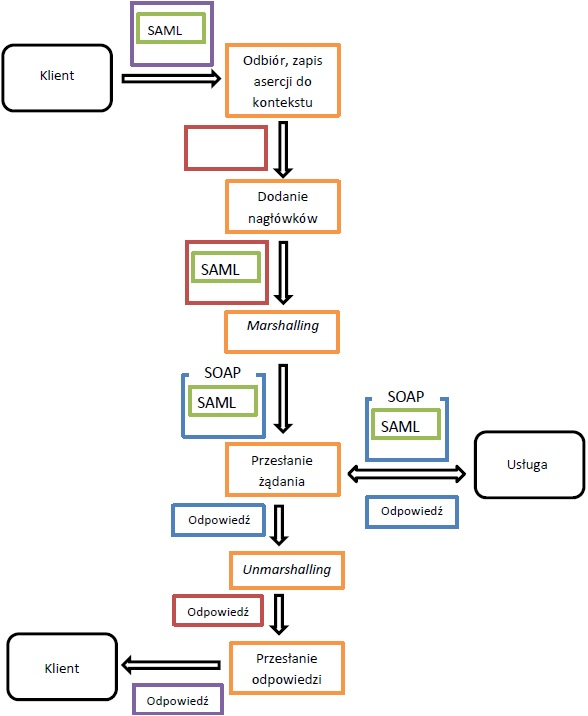
\includegraphics{img/esbRoute.jpg}
		\caption{Implementacja przetwarzania wiadomości przez magistralę usług}
		\label{ESB route}
	\end{figure}

	Klient wywołując usługi przesyła komunikaty określonego formatu - korzystając z określonej metody dostępu do zdalnych serwisów. Moduł magistrali usług otrzymuje komunikat żądania usługi. Do komunikatu dołączony jest nagłówek, w którym przesyłany jest token bezpieczeństwa - asercja SAML. Otrzymany komunikat przekształcany jest do formatu wykorzystywanego wewnętrznie przez moduł przetwarzania wiadomości a informacje zawarte w nagłówku(w tym asercja SAML) zapisywane są w kontekście przetwarzania. Do budowanej wiadomości dodawane są nagłówki(informacje kontekstowe) - dzięki czemu dołączany jest token bezpieczeństwa. Następnie dokonywany jest proces \textit{marshallowania} zbudowanej wiadomości - asercja SAML wpisywana jest do nagłówka(np. SOAP) utworzonego komunikatu. Po serializacji informacji następuje wywołanie usługi korzystające ze zbudowanej wiadomości. Usługa przeprowadza procesy uwierzytelniania klienta i autoryzacji dostępu do zasobów. Po poprawnym przebiegu tych kroków zwracana jest odpowiedź serwisu. Odpowiedź jest \textit{unmarshallowana} i przysłana do klienta w formacie zgodnym z metodą wywołania usługi.
	

%---------------------------------------------------------------------------
